\documentclass{article}
\usepackage{graphicx} % Required for inserting images
\usepackage{tikz}
\usepackage[landscape]{geometry}
\usepackage{float}
\usepackage{listings}

\usetikzlibrary{external}%allows export of pictures
\tikzexternalize 

\usepackage{xcolor}
\definecolor{lgray}{RGB}{200,200,200}
\definecolor{clear}{RGB}{255,255,255}

%arrange page numbers
\usepackage{fancyhdr}
\pagestyle{fancy}
\fancyhf{}
\renewcommand{\headrulewidth}{0pt}
\fancyhead[R]{\thepage}


%load options
\usetikzlibrary{positioning, calc, shapes.geometric, shapes.multipart,
        shapes, arrows.meta, arrows, decorations.markings, external, trees}

%Create custom arrow style:
\tikzstyle{Arrow} = [
thick,
decoration={
markings,
mark=at position 0.9999 with {
\arrow[thick]{latex}}},
shorten >= 3pt, preaction = {decorate}]

\tikzstyle{ArrowRed} = [
ultra thick,
red,
decoration={
markings,
mark=at position 0.9999 with {
\arrow[ultra thick, red]{latex}}},
shorten >= 3pt, preaction = {decorate}]

\tikzstyle{ArrowGray} = [
thick,
lgray,
decoration={
markings,
mark=at position 0.9999 with {
\arrow[thick, lgray]{latex}}},
shorten >= 3pt, preaction = {decorate}]



\title{Box DAGs}
\author{tpfeeney }
\date{June 2023}

\begin{document}

\section{Box DAG}
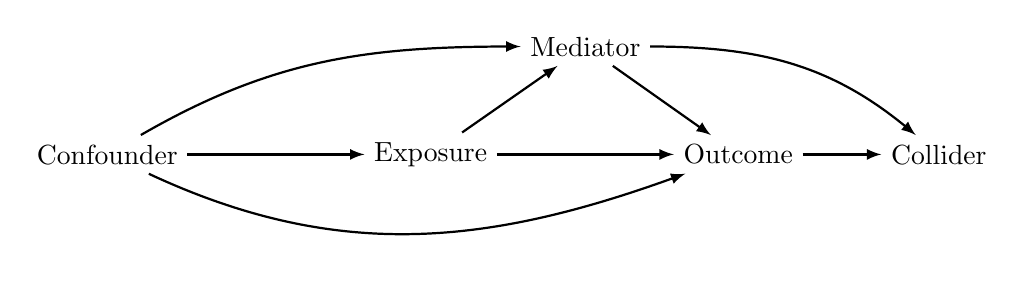
\begin{tikzpicture}
    \node (1) {};
    \node [right =of 1] (2)  {Exposure};
    \node [right =of 2] (3) {};
    \node [right =of 3] (4) {Outcome};
    \node [left =of 1] (5) {Confounder};
    \node [above =of 3] (6) {Mediator};
    \node [right =of 4] (7) {Collider};

    \draw[Arrow] (2.east)--(4.west);
    \draw[Arrow] (2) to (6);
    \draw[Arrow] (6) to (4);
    \draw[Arrow] (5) to [out=-25, in=-160](4);
    \draw[Arrow] (5) to [out=30, in=180] (6);
    \draw[Arrow] (5.east)--(2.west);
    \draw[Arrow] (4.east)--(7.west);
    \draw[Arrow] (6) to [out=0, in=140] (7);
\end{tikzpicture}

\subsection*{node}
\begin{tikzpicture}
    \node (1) {};
    \node [right =of 1] (2)  {Exposure};
    \node [right =of 2] (3) {};
    \node [right =of 3] (4) {Outcome};
    \node [left =of 1] (5) {Confounder};
    \node [above =of 3] (6) {Mediator};
    \node [right =of 4] (7) {Collider};
\end{tikzpicture}

\subsection*{edge}
    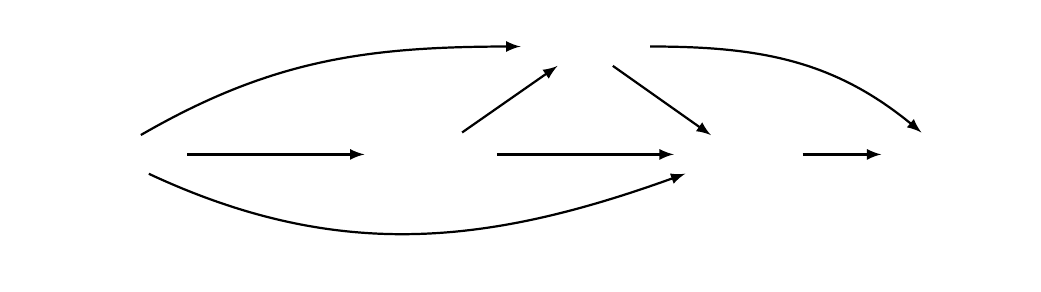
\begin{tikzpicture}
        \node (1) {};
        \node [right =of 1] (2)  {\textcolor{clear}{Exposure}};
        \node [right =of 2] (3) {};
        \node [right =of 3] (4) {\textcolor{clear}{Outcome}};
        \node [left =of 1] (5) {\textcolor{clear}{Confounder}};
        \node [above =of 3] (6) {\textcolor{clear}{Mediator}};
        \node [right =of 4] (7) {\textcolor{clear}{Exposure}};
    
        \draw[Arrow] (2.east)--(4.west);
        \draw[Arrow] (2) to (6);
        \draw[Arrow] (6) to (4);
        \draw[Arrow] (5) to [out=-25, in=-160](4);
        \draw[Arrow] (5) to [out=30, in=180] (6);
        \draw[Arrow] (5.east)--(2.west);
        \draw[Arrow] (4.east)--(7.west);
        \draw[Arrow] (6) to [out=0, in=140] (7);
    \end{tikzpicture}

    
\subsection*{confounder}
\begin{tikzpicture}
    \node (1) {};
    \node [right =of 1] (2)  {Exposure};
    \node [right =of 2] (3) {};
    \node [right =of 3] (4) {Outcome};
    \node [left =of 1] (5) {Confounder};
    \node [above =of 3] (6) {\textcolor{clear}{Mediator}};
    \node [right =of 4] (7) {\textcolor{clear}{Collider}};

    %\draw[Arrow] (2.east)--(4.west);
    %\draw[Arrow] (2) to (6);
    %\draw[Arrow] (6) to (4);
    \draw[Arrow] (5) to [out=-25, in=-160](4);
    %\draw[Arrow] (5) to [out=30, in=180] (6);
    \draw[Arrow] (5.east)--(2.west);
    %\draw[Arrow] (4.east)--(7.west);
    %\draw[Arrow] (6) to [out=0, in=140] (7);
\end{tikzpicture}

\subsection*{mediator; indirect effects}
\begin{tikzpicture}
    \node (1) {};
    \node [right =of 1] (2)  {Exposure};
    \node [right =of 2] (3) {};
    \node [right =of 3] (4) {Outcome};
    \node [left =of 1] (5) {\textcolor{clear}{Confounder}};
    \node [above =of 3] (6) {Mediator};
    \node [right =of 4] (7) {\textcolor{clear}{Collider}};

    %\draw[Arrow] (2.east)--(4.west);
    \draw[Arrow] (2) to (6);
    \draw[Arrow] (6) to (4);
    %\draw[Arrow] (5) to [out=-25, in=-160](4);
    %\draw[Arrow] (5) to [out=30, in=180] (6);
    %\draw[Arrow] (5.east)--(2.west);
    %\draw[Arrow] (4.east)--(7.west);
    %\draw[Arrow] (6) to [out=0, in=140] (7);
\end{tikzpicture}

\subsection*{direct effects}
\begin{tikzpicture}
    \node (1) {};
    \node [right =of 1] (2)  {Exposure};
    \node [right =of 2] (3) {};
    \node [right =of 3] (4) {Outcome};
    \node [left =of 1] (5) {\textcolor{clear}{Confounder}};
    \node [above =of 3] (6) {\textcolor{clear}{Mediator}};
    \node [right =of 4] (7) {\textcolor{clear}{Collider}};

    \draw[Arrow] (2.east)--(4.west);
    %\draw[Arrow] (2) to (6);
    %\draw[Arrow] (6) to (4);
    %\draw[Arrow] (5) to [out=-25, in=-160](4);
    %\draw[Arrow] (5) to [out=30, in=180] (6);
    %\draw[Arrow] (5.east)--(2.west);
    %\draw[Arrow] (4.east)--(7.west);
    %\draw[Arrow] (6) to [out=0, in=140] (7);
\end{tikzpicture}

\subsection*{collider}
\begin{tikzpicture}
    \node (1) {};
    \node [right =of 1] (2)  {\textcolor{clear}{Exposure}};
    \node [right =of 2] (3) {};
    \node [right =of 3] (4) {\textcolor{clear}{Outcome}};
    \node [left =of 1] (5) {\textcolor{clear}{Confounder}};
    \node [above =of 3] (6) {\textcolor{clear}{Mediator}};
    \node [right =of 4] (7) {Collider};

    %\draw[Arrow] (2.east)--(4.west);
    %\draw[Arrow] (2) to (6);
    %\draw[Arrow] (6) to (4);
    %\draw[Arrow] (5) to [out=-25, in=-160](4);
    %\draw[Arrow] (5) to [out=30, in=180] (6);
    %\draw[Arrow] (5.east)--(2.west);
    \draw[Arrow] (4.east)--(7.west);
    \draw[Arrow] (6) to [out=0, in=140] (7);
\end{tikzpicture}



%%%%%%%%%%%%%%%%%%%%
%ALTERNATIVES%
%%%%%%%%%%%%%%%%%%%%%

\subsection*{Nodes}
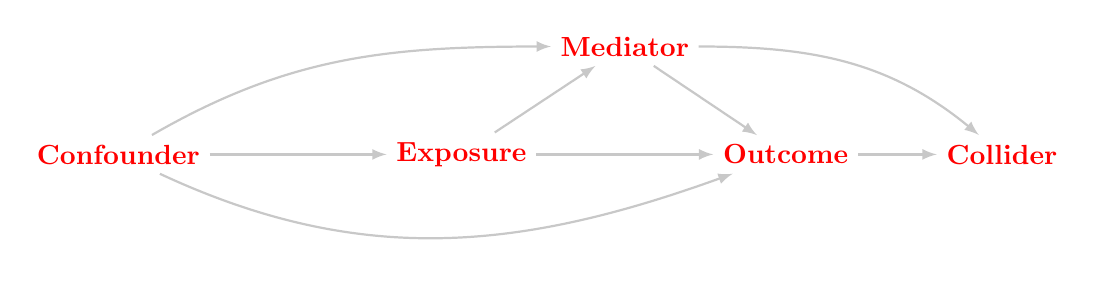
\begin{tikzpicture}
    \node (1) {};
    \node [right =of 1] (2)  {\textcolor{red}{\textbf{Exposure}}};
    \node [right =of 2] (3) {};
    \node [right =of 3] (4) {\textcolor{red}{\textbf{Outcome}}};
    \node [left =of 1] (5) {\textcolor{red}{\textbf{Confounder}}};
    \node [above =of 3] (6) {\textcolor{red}{\textbf{Mediator}}};
    \node [right =of 4] (7) {\textcolor{red}{\textbf{Collider}}};

    \draw[ArrowGray] (2.east)--(4.west);
    \draw[ArrowGray] (2) to (6);
    \draw[ArrowGray] (6) to (4);
    \draw[ArrowGray] (5) to [out=-25, in=-160](4);
    \draw[ArrowGray] (5) to [out=30, in=180] (6);
    \draw[ArrowGray] (5.east)--(2.west);
    \draw[ArrowGray] (4.east)--(7.west);
    \draw[ArrowGray] (6) to [out=0, in=140] (7);
\end{tikzpicture}

\subsection*{Edges}
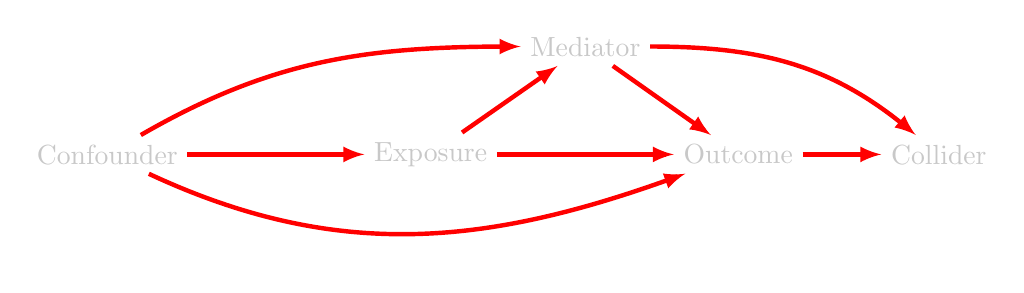
\begin{tikzpicture}
    \node (1) {};
    \node [right =of 1] (2)  {\textcolor{lgray}{Exposure}};
    \node [right =of 2] (3) {};
    \node [right =of 3] (4) {\textcolor{lgray}{Outcome}};
    \node [left =of 1] (5) {\textcolor{lgray}{Confounder}};
    \node [above =of 3] (6) {\textcolor{lgray}{Mediator}};
    \node [right =of 4] (7) {\textcolor{lgray}{Collider}};

    \draw[ArrowRed] (2.east)--(4.west);
    \draw[ArrowRed] (2) to (6);
    \draw[ArrowRed] (6) to (4);
    \draw[ArrowRed] (5) to [out=-25, in=-160](4);
    \draw[ArrowRed] (5) to [out=30, in=180] (6);
    \draw[ArrowRed] (5.east)--(2.west);
    \draw[ArrowRed] (4.east)--(7.west);
    \draw[ArrowRed] (6) to [out=0, in=140] (7);
\end{tikzpicture}


\subsection*{Confounder}
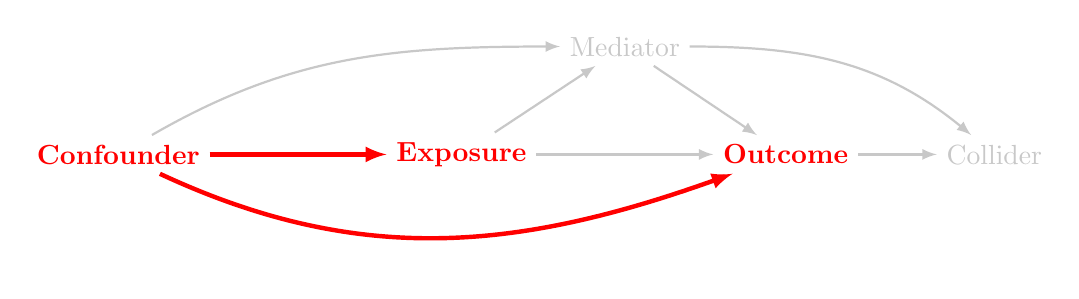
\begin{tikzpicture}
    \node (1) {};
    \node [right =of 1] (2)  {\textcolor{red}{\textbf{Exposure}}};
    \node [right =of 2] (3) {};
    \node [right =of 3] (4) {\textcolor{red}{\textbf{Outcome}}};
    \node [left =of 1] (5) {\textcolor{red}{\textbf{Confounder}}};
    \node [above =of 3] (6) {\textcolor{lgray}{Mediator}};
    \node [right =of 4] (7) {\textcolor{lgray}{Collider}};

    \draw[ArrowGray] (2.east)--(4.west);
    \draw[ArrowGray] (2) to (6);
    \draw[ArrowGray] (6) to (4);
    \draw[ArrowRed] (5) to [out=-25, in=-160](4);
    \draw[ArrowGray] (5) to [out=30, in=180] (6);
    \draw[ArrowRed] (5.east)--(2.west);
    \draw[ArrowGray] (4.east)--(7.west);
    \draw[ArrowGray] (6) to [out=0, in=140] (7);
\end{tikzpicture}

\subsection*{Indirect Effects/Mediator}
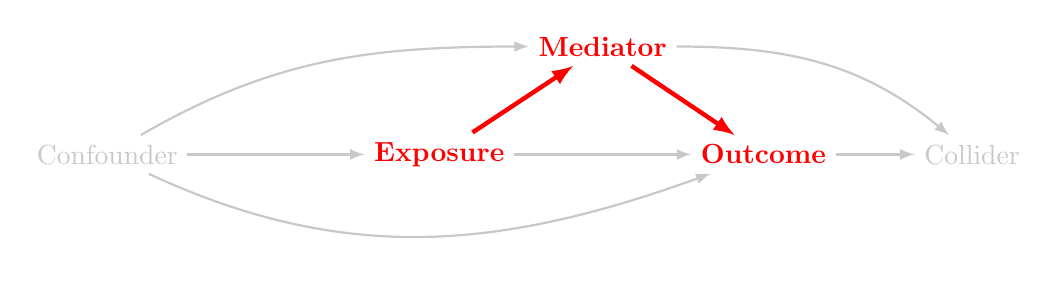
\begin{tikzpicture}
    \node (1) {};
    \node [right =of 1] (2)  {\textcolor{red}{\textbf{Exposure}}};
    \node [right =of 2] (3) {};
    \node [right =of 3] (4) {\textcolor{red}{\textbf{Outcome}}};
    \node [left =of 1] (5) {\textcolor{lgray}{Confounder}};
    \node [above =of 3] (6) {\textcolor{red}{\textbf{Mediator}}};
    \node [right =of 4] (7) {\textcolor{lgray}{Collider}};

    \draw[ArrowGray] (2.east)--(4.west);
    \draw[ArrowRed] (2) to (6);
    \draw[ArrowRed] (6) to (4);
    \draw[ArrowGray] (5) to [out=-25, in=-160](4);
    \draw[ArrowGray] (5) to [out=30, in=180] (6);
    \draw[ArrowGray] (5.east)--(2.west);
    \draw[ArrowGray] (4.east)--(7.west);
    \draw[ArrowGray] (6) to [out=0, in=140] (7);
\end{tikzpicture}

\subsection*{Direct Effects}
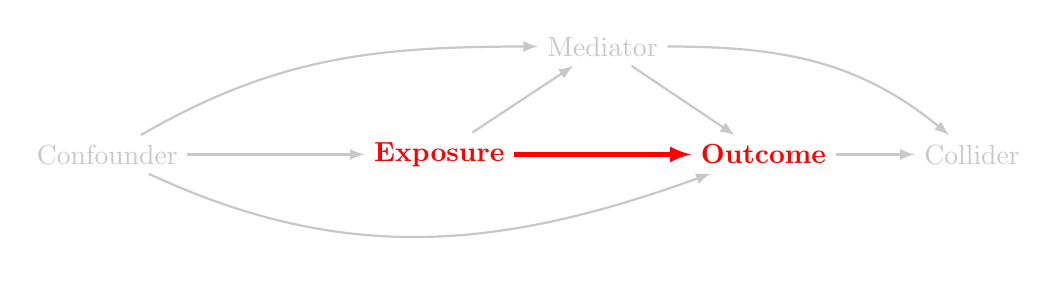
\begin{tikzpicture}
    \node (1) {};
    \node [right =of 1] (2)  {\textcolor{red}{\textbf{Exposure}}};
    \node [right =of 2] (3) {};
    \node [right =of 3] (4) {\textcolor{red}{\textbf{Outcome}}};
    \node [left =of 1] (5) {\textcolor{lgray}{Confounder}};
    \node [above =of 3] (6) {\textcolor{lgray}{Mediator}};
    \node [right =of 4] (7) {\textcolor{lgray}{Collider}};

    \draw[ArrowRed] (2.east)--(4.west);
    \draw[ArrowGray] (2) to (6);
    \draw[ArrowGray] (6) to (4);
    \draw[ArrowGray] (5) to [out=-25, in=-160](4);
    \draw[ArrowGray] (5) to [out=30, in=180] (6);
    \draw[ArrowGray] (5.east)--(2.west);
    \draw[ArrowGray] (4.east)--(7.west);
    \draw[ArrowGray] (6) to [out=0, in=140] (7);
\end{tikzpicture}

\subsection*{Collider}
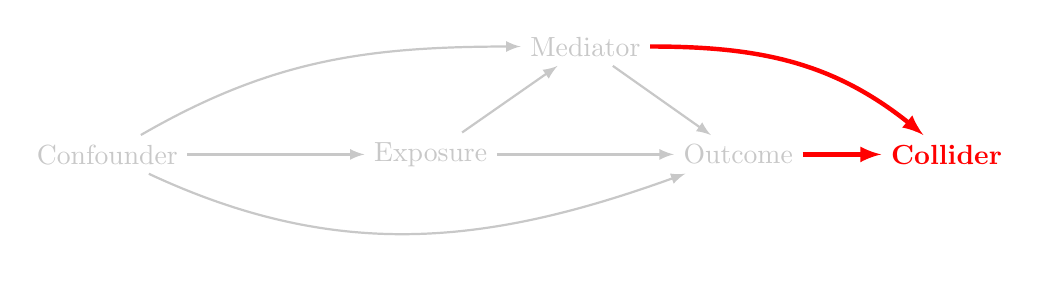
\begin{tikzpicture}
    \node (1) {};
    \node [right =of 1] (2)  {\textcolor{lgray}{Exposure}};
    \node [right =of 2] (3) {};
    \node [right =of 3] (4) {\textcolor{lgray}{Outcome}};
    \node [left =of 1] (5) {\textcolor{lgray}{Confounder}};
    \node [above =of 3] (6) {\textcolor{lgray}{Mediator}};
    \node [right =of 4] (7) {\textcolor{red}{\textbf{Collider}}};

    \draw[ArrowGray] (2.east)--(4.west);
    \draw[ArrowGray] (2) to (6);
    \draw[ArrowGray] (6) to (4);
    \draw[ArrowGray] (5) to [out=-25, in=-160](4);
    \draw[ArrowGray] (5) to [out=30, in=180] (6);
    \draw[ArrowGray] (5.east)--(2.west);
    \draw[ArrowRed] (4.east)--(7.west);
    \draw[ArrowRed] (6) to [out=0, in=140] (7);
\end{tikzpicture}

\end{document}
